\documentclass[10pt]{article}
\usepackage[T1]{fontenc}\usepackage{times}
\usepackage[margin=0.8in]{geometry}
\usepackage{amsmath,graphicx,longtable}
\ifdefined\pdfinfo\pdfinfo{/Author (EurekaChen) /Title () /Subject () /Keywords ()}
\else\special{pdf:docinfo << /Author (EurekaChen) /Title () /Subject () /Keywords () >>}\fi
\title{Appendix: Clinical-Anchored Multi-Omics Graph Learning}
\author{Author information to be completed}\date{}
\begin{document}\pagestyle{empty}\maketitle\thispagestyle{empty}
This is a separate author-review supplement. It is not part of the four-page
ISBI manuscript and is not assumed eligible for extra technical submission pages.
\section{Data alignment and evidence boundaries}
The primary cohort contains 1,416 unique primary-tumour patients with three
molecular assays and valid overall survival; 830 died. Clinical records numbered
2,509, and 1,980 had usable survival. Three assay intersections contained 1,417
clinical samples before survival/primary-tumour filtering. The clinical-table
exclusions therefore total 1,093 for the final complete-assay analysis.
Source-file hashes and exact feature counts are in results/data\_audit.json.
No outcomes, recurrence fields, future treatment information or cohort labels
are used as predictive clinical inputs. Cohort labels are reserved for evaluation.

The supplied TCGA/MOGONET matrices lack patient IDs and are not joined by row
order to METABRIC. BUSI and BUSBRA are unrelated patients and are not joined
to molecular records. CNA replaces the preliminary miRNA view. Temporal
graphs, simulated visits, clinical notes and paired imaging are not evaluated.

\begin{center}
\footnotesize
\begin{tabular}{lrr}\hline
Source group & Patients & Deaths\\\hline
1.000 & 386.000 & 173.000\\
2.000 & 225.000 & 121.000\\
3.000 & 495.000 & 357.000\\
4.000 & 160.000 & 80.000\\
5.000 & 150.000 & 99.000\\
\hline\end{tabular}
\end{center}
\begin{center}
\footnotesize
\begin{tabular}{lrr}\hline
View & Raw features & Missing cells\\\hline
mRNA & 20603 & 10\\
Methylation & 13188 & 553726\\
CNA & 22544 & 557\\
\hline\end{tabular}
\end{center}
\section{All fixed parameters and search settings}
\begin{longtable}{p{.48\textwidth}p{.43\textwidth}}\hline Parameter & Value\\\hline
outer\_folds & 5\\
validation\_fraction & 0.2\\
split\_seed & 42\\
seeds & [42, 2026, 3407]\\
trials & 12\\
epochs & 300\\
patience & 30\\
bootstrap & 1000\\
confidence\_level & 0.95\\
concordance\_tie\_tolerance & 1e-08\\
prediction\_horizons\_months & [12, 36, 60]\\
ipcw\_tau\_training\_quantile & 0.9\\
minimum\_censoring\_survival & 0.05\\
calibration\_bins & 5\\
risk\_group\_rule & "training median per fold and seed; three-seed majority vote"\\
feature\_counts & [500, 1000]\\
ranks & [4, 8, 16]\\
ridges & [0.01, 0.1, 1.0]\\
anchors & [1.0, 2.0]\\
neighbors & [5, 10, 20]\\
hidden\_sizes & [32, 64]\\
learning\_rates & [0.001, 0.003, 0.01]\\
mask\_rates & [0.0, 0.2, 0.4]\\
dropout & 0.3\\
gcn\_layers & 2\\
activation & "ReLU"\\
layernorm\_epsilon & 1e-05\\
weight\_decay & 0.001\\
optimizer & "AdamW"\\
optimizer\_betas & [0.9, 0.999]\\
optimizer\_epsilon & 1e-08\\
scheduler & "none"\\
gradient\_clip & 5.0\\
empty\_mask\_fallback & "mRNA retained"\\
cox\_ties & "Breslow"\\
gcca\_centering & "training mean"\\
gcca\_projection\_scaling & "training standard deviation"\\
graph\_metric & "cosine"\\
graph\_adjacency & "symmetric binary training kNN with self loops"\\
query\_edges & "training to query only; frozen reference states and degrees"\\
feature\_max\_missing\_fraction & 0.2\\
feature\_clip\_standard\_deviations & 5.0\\
methylation\_epsilon & 1e-05\\
tfidf\_min\_df & 2\\
tfidf\_max\_features & 10000\\
tfidf\_ngram\_range & [1, 2]\\
tfidf\_norm & "l2"\\
tfidf\_lowercase & true\\
tfidf\_smooth\_idf & true\\
tfidf\_sublinear\_tf & false\\
text\_svd\_max\_dimensions & 128\\
cox\_l1\_ratio & 0.1\\
cox\_max\_iterations & 10000\\
cox\_tolerance & 1e-06\\
rsf\_trees & 200\\
rsf\_jobs & 4\\
rsf\_low\_memory & true\\
rsf\_survival & "bootstrap-weighted terminal-node Kaplan-Meier; native-equivalence tested"\\
rsf\_max\_features & "sqrt"\\
multisurv\_encoder\_dimensions & [128, 32]\\
multisurv\_intervals & 30\\
multisurv\_interval\_months & 12\\
integrao\_fusing\_iterations & 20\\
integrao\_alignment\_epochs & 300\\
integrao\_hidden & 128\\
integrao\_embedding & 8\\
integrao\_neighbors & 10\\
integrao\_cox\_tolerance & 1e-07\\
threads & 2\\
\hline\end{longtable}
The twelve candidate dictionaries are in search\_candidates.json;
selected\_parameters.csv stores the actual fold/seed settings. GCCA projection
coordinates are standardized using training projection standard deviations.
Clinical numerical values are inserted into fixed field--value templates;
missing values are ``unknown''. Structured clinical encoding uses training
median filling, numerical missingness indicators, standardization and one-hot
categories with unknown categories ignored. TF-IDF retains tokens containing
digits and decimals; no pretrained language encoder is used.

Coxnet uses l1 ratio 0.1, at most 10,000 iterations and tolerance $10^{-6}$.
Its size is the number of nonzero coefficients. Neural size is the number of
trainable scalar parameters. Survival-forest size is total tree-node count,
which is not directly comparable to neural parameter count. The forest uses
200 trees, square-root feature sampling and four local workers. Its memory-
efficient implementation reconstructs terminal-node bootstrap-weighted
Kaplan--Meier probabilities only at requested horizons; agreement with native
full-memory survival curves is tested. Twelve configurations are an upper budget, not an
exhaustive Cartesian search. Some candidate choices irrelevant to a particular
baseline are retained in the audit record but do not change that model;
duplicate effective forest configurations are evaluated once. The structured
clinical Cox control was added after initial fold inspection to strengthen
the clinical comparison. This is an exploratory, non-preregistered study.

MultiSurv-style encoders have a 128-unit first layer and 32/64-unit output,
elementwise maximum fusion and a same-width hidden prediction layer producing
30 twelve-month hazards. Its scalar C-index risk is negative summed survival
across intervals, whereas time-dependent AUC below uses this same global marker.
Its original pan-cancer architecture and original code are not reproduced exactly.
MOGONET-style encoders use modality-specific two-layer graphs and a concatenated
Cox head; no classification-label VCDN is used. DeepSurv-style denotes a
two-hidden-layer ReLU/dropout MLP trained with Cox loss.

IntegrAO uses the official 0.1.3 implementation with fixed representation
settings: 128 hidden units, 8 output dimensions, 10 neighbors, 20 diffusion
steps, and 300 alignment epochs. Adam uses its original schedule from 0.1,
decayed by ten each 100 epochs to a minimum 0.001; alignment MSE weight is
one and t-SNE early exaggeration is removed at epoch 100. A Coxnet head alpha
is selected from twelve log-spaced values $10^{-3}$ to $10^1$; its Coxnet
head uses tolerance $10^{-7}$ (the other Coxnet baselines use $10^{-6}$). New patients
receive one-way incoming edges from training neighbors only. Evaluation mode
freezes batch normalization; query-batch independence is asserted. These
survival and inductive adapters are explicit departures from the original
downstream task. Exact package versions are in requirements.txt and environment.json.

\section{Full discrimination, time-dependent metrics and model size}
\begin{center}
\footnotesize
\begin{tabular}{lrrr}\hline
Configuration & C-index & CI low & CI high\\\hline
Structured clinical Cox & 0.656 & 0.634 & 0.675\\
Structured clinical input & 0.655 & 0.635 & 0.672\\
Random survival forest & 0.620 & 0.600 & 0.639\\
mRNA Cox & 0.619 & 0.599 & 0.640\\
Pairwise CCA + Cox & 0.619 & 0.599 & 0.639\\
Templated clinical Cox & 0.618 & 0.596 & 0.638\\
Without raw residual & 0.609 & 0.590 & 0.627\\
DeepSurv-style MLP & 0.607 & 0.587 & 0.626\\
Shared-anchor GCCA + graph & 0.607 & 0.587 & 0.625\\
MOGONET-style + Cox & 0.605 & 0.585 & 0.625\\
Concatenation Cox & 0.604 & 0.584 & 0.625\\
Without graph & 0.602 & 0.582 & 0.620\\
Equal GCCA weights & 0.601 & 0.581 & 0.619\\
GCCA + Cox & 0.598 & 0.576 & 0.621\\
Without view masking & 0.597 & 0.577 & 0.616\\
Original pairwise CCA + graph & 0.591 & 0.575 & 0.609\\
MultiSurv-style (scaled) & 0.586 & 0.567 & 0.605\\
Official IntegrAO + Cox adapter & 0.576 & 0.557 & 0.597\\
Methylation Cox & 0.544 & 0.523 & 0.567\\
CNA Cox & 0.515 & 0.492 & 0.538\\
\hline\end{tabular}
\end{center}
\begin{center}
\footnotesize
\begin{tabular}{lrrrr}\hline
Configuration & IPCW C & AUC 1y & AUC 3y & AUC 5y\\\hline
Structured clinical Cox & 0.654 & 0.733 & 0.674 & 0.687\\
Structured clinical input & 0.645 & 0.650 & 0.680 & 0.688\\
Random survival forest & 0.600 & 0.796 & 0.678 & 0.669\\
mRNA Cox & 0.607 & 0.580 & 0.655 & 0.661\\
Pairwise CCA + Cox & 0.603 & 0.598 & 0.658 & 0.651\\
Templated clinical Cox & 0.605 & 0.747 & 0.678 & 0.666\\
Without raw residual & 0.594 & 0.601 & 0.668 & 0.655\\
DeepSurv-style MLP & 0.597 & 0.650 & 0.633 & 0.645\\
Shared-anchor GCCA + graph & 0.590 & 0.671 & 0.669 & 0.652\\
MOGONET-style + Cox & 0.595 & 0.731 & 0.640 & 0.638\\
Concatenation Cox & 0.592 & 0.741 & 0.638 & 0.631\\
Without graph & 0.586 & 0.691 & 0.666 & 0.647\\
Equal GCCA weights & 0.586 & 0.661 & 0.652 & 0.648\\
GCCA + Cox & 0.581 & 0.679 & 0.665 & 0.639\\
Without view masking & 0.583 & 0.708 & 0.659 & 0.643\\
Original pairwise CCA + graph & 0.579 & 0.640 & 0.639 & 0.617\\
MultiSurv-style (scaled) & 0.576 & 0.623 & 0.593 & 0.607\\
Official IntegrAO + Cox adapter & 0.556 & 0.626 & 0.641 & 0.628\\
Methylation Cox & 0.543 & 0.623 & 0.524 & 0.542\\
CNA Cox & 0.512 & 0.451 & 0.547 & 0.531\\
\hline\end{tabular}
\end{center}
\begin{center}
\footnotesize
\begin{tabular}{lrrrr}\hline
Configuration & BS 1y & BS 3y & BS 5y & Size\\\hline
Structured clinical Cox & 0.015 & 0.091 & 0.157 & 22.000\\
Structured clinical input & 0.015 & 0.091 & 0.158 & 11045.000\\
Random survival forest & 0.015 & 0.090 & 0.161 & 17614.000\\
mRNA Cox & 0.015 & 0.096 & 0.165 & 472.000\\
Pairwise CCA + Cox & 0.015 & 0.093 & 0.167 & 14.000\\
Templated clinical Cox & 0.015 & 0.093 & 0.163 & 83.000\\
Without raw residual & 0.015 & 0.093 & 0.165 & 11009.000\\
DeepSurv-style MLP & 0.015 & 0.097 & 0.176 & 204481.000\\
Shared-anchor GCCA + graph & 0.015 & 0.092 & 0.164 & 11045.000\\
MOGONET-style + Cox & 0.015 & 0.094 & 0.171 & 121345.000\\
Concatenation Cox & 0.017 & 0.111 & 0.198 & 465.000\\
Without graph & 0.015 & 0.092 & 0.166 & 11045.000\\
Equal GCCA weights & 0.015 & 0.093 & 0.165 & 11045.000\\
GCCA + Cox & 0.015 & 0.092 & 0.165 & 19.000\\
Without view masking & 0.015 & 0.093 & 0.167 & 11045.000\\
Original pairwise CCA + graph & 0.015 & 0.096 & 0.180 & 10005.000\\
MultiSurv-style (scaled) & 0.015 & 0.094 & 0.174 & 419454.000\\
Official IntegrAO + Cox adapter & 0.015 & 0.094 & 0.169 & 809664.000\\
Methylation Cox & 0.024 & 0.148 & 0.241 & 401.000\\
CNA Cox & 0.017 & 0.106 & 0.188 & 420.000\\
\hline\end{tabular}
\end{center}
Harrell concordance is the mean across five held-out folds and
three seeds. Intervals use 1,000 patient-level bootstrap resamples separately
within each held-out fold, with identical resamples for all methods. Seed-wise
concordance contributions are averaged within a resample. These intervals are
conditional on fitted models, not nested-bootstrap retraining intervals.
Pairwise differences are two-sided and Holm-adjusted over all comparisons
against the proposed configuration, including ablations. Raw test outcomes
are retained for Harrell concordance. For time-dependent metrics, follow-up
beyond training support is administratively censored just below the largest
training follow-up. Censoring survival at each horizon must exceed 0.05; a
nonestimable metric is NA. Fold-average time-dependent metrics use available
estimable folds. No finite-sample selective-risk guarantee is inferred.

\begin{center}
\footnotesize
\begin{tabular}{lrrrr}\hline
Comparator & Difference & CI low & CI high & Holm p\\\hline
Methylation Cox & 0.063 & 0.038 & 0.088 & 0.038\\
CNA Cox & 0.092 & 0.066 & 0.118 & 0.038\\
Structured clinical input & -0.048 & -0.065 & -0.031 & 0.038\\
Structured clinical Cox & -0.049 & -0.075 & -0.025 & 0.038\\
Official IntegrAO + Cox adapter & 0.031 & 0.010 & 0.052 & 0.060\\
Without view masking & 0.009 & 0.003 & 0.015 & 0.060\\
MultiSurv-style (scaled) & 0.021 & 0.001 & 0.041 & 0.519\\
Without graph & 0.005 & -0.000 & 0.011 & 0.839\\
Original pairwise CCA + graph & 0.015 & -0.003 & 0.035 & 1.000\\
Equal GCCA weights & 0.006 & -0.002 & 0.013 & 1.000\\
Random survival forest & -0.012 & -0.031 & 0.005 & 1.000\\
Pairwise CCA + Cox & -0.012 & -0.031 & 0.007 & 1.000\\
mRNA Cox & -0.012 & -0.033 & 0.009 & 1.000\\
Templated clinical Cox & -0.011 & -0.034 & 0.012 & 1.000\\
GCCA + Cox & 0.008 & -0.009 & 0.026 & 1.000\\
Without raw residual & -0.002 & -0.008 & 0.004 & 1.000\\
Concatenation Cox & 0.003 & -0.019 & 0.025 & 1.000\\
MOGONET-style + Cox & 0.002 & -0.017 & 0.021 & 1.000\\
DeepSurv-style MLP & -0.000 & -0.019 & 0.018 & 1.000\\
\hline\end{tabular}
\end{center}
\section{All missing-view combinations}
\begin{center}
\footnotesize
\begin{tabular}{lrrr}\hline
mRNA/Meth/CNA/Clinical & Proposed & Pairwise graph & No masking\\\hline
0001 & 0.587 & 0.562 & 0.578\\
0010 & 0.531 & 0.522 & 0.512\\
0011 & 0.577 & 0.560 & 0.562\\
0100 & 0.547 & 0.504 & 0.534\\
0101 & 0.596 & 0.549 & 0.584\\
0110 & 0.541 & 0.510 & 0.522\\
0111 & 0.579 & 0.545 & 0.564\\
1000 & 0.598 & 0.590 & 0.587\\
1001 & 0.613 & 0.597 & 0.608\\
1010 & 0.590 & 0.589 & 0.575\\
1011 & 0.604 & 0.598 & 0.595\\
1100 & 0.602 & 0.581 & 0.591\\
1101 & 0.617 & 0.591 & 0.609\\
1110 & 0.592 & 0.578 & 0.578\\
1111 & 0.607 & 0.591 & 0.597\\
\hline\end{tabular}
\end{center}
\begin{center}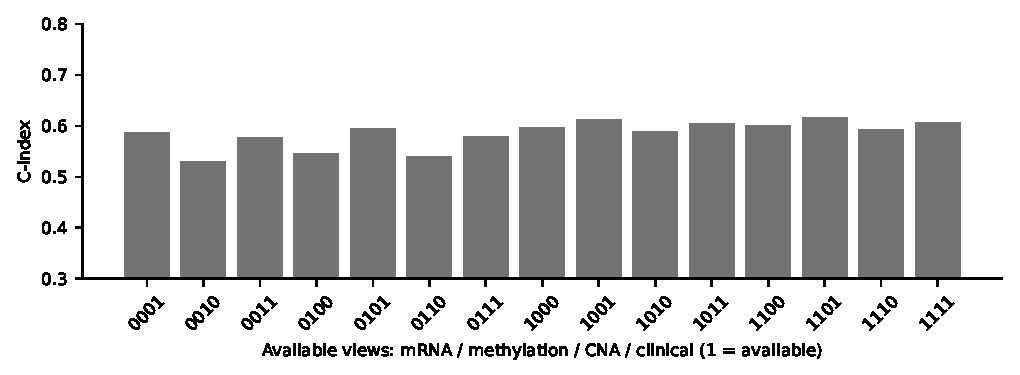
\includegraphics[width=.9\textwidth]{missing.pdf}\end{center}
\begin{center}
\footnotesize
\begin{tabular}{lrr}\hline
Configuration & Missing probability & C-index\\\hline
Without view masking & 0.100 & 0.591\\
Without view masking & 0.300 & 0.584\\
Without view masking & 0.500 & 0.568\\
Original pairwise CCA + graph & 0.100 & 0.587\\
Original pairwise CCA + graph & 0.300 & 0.574\\
Original pairwise CCA + graph & 0.500 & 0.565\\
Shared-anchor GCCA + graph & 0.100 & 0.599\\
Shared-anchor GCCA + graph & 0.300 & 0.599\\
Shared-anchor GCCA + graph & 0.500 & 0.587\\
\hline\end{tabular}
\end{center}
\section{Source-group holdouts}
\subsection{cohort1}
\begin{center}
\footnotesize
\begin{tabular}{lrrrr}\hline
Configuration & Patients & Deaths & C-index & Seed SD\\\hline
Templated clinical Cox & 386 & 173 & 0.612 & 0.000\\
Structured clinical Cox & 386 & 173 & 0.722 & 0.000\\
Concatenation Cox & 386 & 173 & 0.620 & 0.000\\
GCCA + Cox & 386 & 173 & 0.667 & 0.000\\
Official IntegrAO + Cox adapter & 386 & 173 & 0.609 & 0.009\\
Original pairwise CCA + graph & 386 & 173 & 0.653 & 0.034\\
Shared-anchor GCCA + graph & 386 & 173 & 0.658 & 0.019\\
\hline\end{tabular}
\end{center}
\subsection{cohort2}
\begin{center}
\footnotesize
\begin{tabular}{lrrrr}\hline
Configuration & Patients & Deaths & C-index & Seed SD\\\hline
Templated clinical Cox & 225 & 121 & 0.612 & 0.000\\
Structured clinical Cox & 225 & 121 & 0.605 & 0.000\\
Concatenation Cox & 225 & 121 & 0.604 & 0.000\\
GCCA + Cox & 225 & 121 & 0.611 & 0.000\\
Official IntegrAO + Cox adapter & 225 & 121 & 0.584 & 0.008\\
Original pairwise CCA + graph & 225 & 121 & 0.552 & 0.019\\
Shared-anchor GCCA + graph & 225 & 121 & 0.607 & 0.016\\
\hline\end{tabular}
\end{center}
\subsection{cohort3}
\begin{center}
\footnotesize
\begin{tabular}{lrrrr}\hline
Configuration & Patients & Deaths & C-index & Seed SD\\\hline
Templated clinical Cox & 495 & 357 & 0.594 & 0.000\\
Structured clinical Cox & 495 & 357 & 0.620 & 0.000\\
Concatenation Cox & 495 & 357 & 0.581 & 0.000\\
GCCA + Cox & 495 & 357 & 0.575 & 0.000\\
Official IntegrAO + Cox adapter & 495 & 357 & 0.556 & 0.009\\
Original pairwise CCA + graph & 495 & 357 & 0.567 & 0.011\\
Shared-anchor GCCA + graph & 495 & 357 & 0.584 & 0.003\\
\hline\end{tabular}
\end{center}
\subsection{cohort4}
\begin{center}
\footnotesize
\begin{tabular}{lrrrr}\hline
Configuration & Patients & Deaths & C-index & Seed SD\\\hline
Templated clinical Cox & 160 & 80 & 0.593 & 0.000\\
Structured clinical Cox & 160 & 80 & 0.659 & 0.000\\
Concatenation Cox & 160 & 80 & 0.651 & 0.000\\
GCCA + Cox & 160 & 80 & 0.624 & 0.000\\
Official IntegrAO + Cox adapter & 160 & 80 & 0.600 & 0.014\\
Original pairwise CCA + graph & 160 & 80 & 0.611 & 0.025\\
Shared-anchor GCCA + graph & 160 & 80 & 0.641 & 0.016\\
\hline\end{tabular}
\end{center}
\subsection{cohort5}
\begin{center}
\footnotesize
\begin{tabular}{lrrrr}\hline
Configuration & Patients & Deaths & C-index & Seed SD\\\hline
Templated clinical Cox & 150 & 99 & 0.558 & 0.000\\
Structured clinical Cox & 150 & 99 & 0.630 & 0.000\\
Concatenation Cox & 150 & 99 & 0.574 & 0.000\\
GCCA + Cox & 150 & 99 & 0.540 & 0.000\\
Official IntegrAO + Cox adapter & 150 & 99 & 0.526 & 0.010\\
Original pairwise CCA + graph & 150 & 99 & 0.552 & 0.011\\
Shared-anchor GCCA + graph & 150 & 99 & 0.562 & 0.014\\
\hline\end{tabular}
\end{center}
These are leave-one-source-group-out analyses within METABRIC,
not independently collected external cohorts. Their preprocessing and graph
references exclude the held-out group. Validation is 20\% of remaining patients,
event-stratified with seed 42. The same 12-configuration upper search budget
is used except for the documented fixed IntegrAO representation.
\section{Calibration, risk groups and interpretability limits}
\begin{center}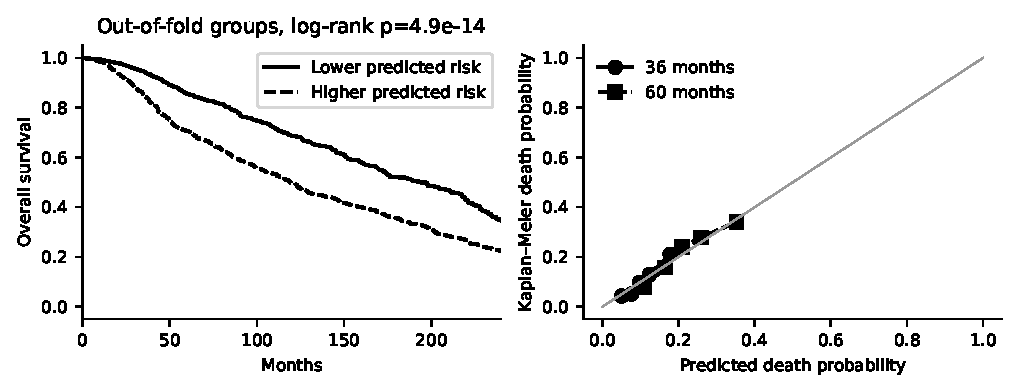
\includegraphics[width=.95\textwidth]{calibration_km.pdf}\end{center}
Each training fold's median predicted risk defines its test high-risk group;
three seed-wise decisions are combined by majority vote. Calibration averages
the three seed-specific survival probabilities within each held-out fold,
then compares prediction quintiles with Kaplan--Meier event probabilities.
These plots are descriptive, and risk-group separation is not a replacement
for discrimination or calibration metrics. GCCA loadings are linear
associations and should not be described as causal biomarkers. The current
study does not establish clinically validated biomarkers or graph attention:
the implemented graph is a GCN, not an attention network.

\section{Relationship to supplied reference PDFs}
The CXR-LT reports (Holste 2024; Dong 2026 overview and full report) concern
long-tailed chest-X-ray classification. They motivate careful cross-domain
testing but do not supply survival comparison numbers. The Aperstein 2025
preprint and 2026 Scientific Reports version concern rejection in
multi-pathology chest-X-ray classification; the later article is not counted
as an independent second study. Geifman and El-Yaniv (2017) concerns selective
classification. Bates et al. (2021) concerns risk-controlling prediction sets;
Angelopoulos et al. (Learn Then Test, arXiv 2021) concerns finite-sample
calibration through hypothesis testing. Their guarantees are not transferred
to censored Cox outcomes in this implementation. No chest-X-ray experiment,
selective survival guarantee, or numerical baseline result is invented.

\section{Per-fold audit and reproducibility}
The complete fold-results CSV contains all patient counts, event counts,
metrics, training seconds, selected epoch, model size and exact configuration.
All forty selected main-CV Cox solutions were re-fitted in a convergence
audit. They reproduced their original C-indices to numerical precision and
emitted no solver warnings. Failed numerical search candidates were not
assigned performance values and were excluded from selection; the attempt
log retains their status. Interrupted, uncompleted fits were rerun.
The following table includes each completed main-CV fold/seed result.

\begin{longtable}{llrrr}\hline Configuration & Fold & Seed & C-index & Epoch\\\hline
clinical\_cox & cv0 & 42 & 0.6354 & 0\\
clinical\_cox & cv0 & 2026 & 0.6354 & 0\\
clinical\_cox & cv0 & 3407 & 0.6354 & 0\\
clinical\_cox & cv1 & 42 & 0.5896 & 0\\
clinical\_cox & cv1 & 2026 & 0.5896 & 0\\
clinical\_cox & cv1 & 3407 & 0.5896 & 0\\
clinical\_cox & cv2 & 42 & 0.5985 & 0\\
clinical\_cox & cv2 & 2026 & 0.5985 & 0\\
clinical\_cox & cv2 & 3407 & 0.5985 & 0\\
clinical\_cox & cv3 & 42 & 0.6290 & 0\\
clinical\_cox & cv3 & 2026 & 0.6290 & 0\\
clinical\_cox & cv3 & 3407 & 0.6290 & 0\\
clinical\_cox & cv4 & 42 & 0.6395 & 0\\
clinical\_cox & cv4 & 2026 & 0.6395 & 0\\
clinical\_cox & cv4 & 3407 & 0.6395 & 0\\
clinical\_structured\_cox & cv0 & 42 & 0.6479 & 0\\
clinical\_structured\_cox & cv0 & 2026 & 0.6479 & 0\\
clinical\_structured\_cox & cv0 & 3407 & 0.6479 & 0\\
clinical\_structured\_cox & cv1 & 42 & 0.6453 & 0\\
clinical\_structured\_cox & cv1 & 2026 & 0.6453 & 0\\
clinical\_structured\_cox & cv1 & 3407 & 0.6453 & 0\\
clinical\_structured\_cox & cv2 & 42 & 0.6487 & 0\\
clinical\_structured\_cox & cv2 & 2026 & 0.6487 & 0\\
clinical\_structured\_cox & cv2 & 3407 & 0.6487 & 0\\
clinical\_structured\_cox & cv3 & 42 & 0.6772 & 0\\
clinical\_structured\_cox & cv3 & 2026 & 0.6772 & 0\\
clinical\_structured\_cox & cv3 & 3407 & 0.6772 & 0\\
clinical\_structured\_cox & cv4 & 42 & 0.6601 & 0\\
clinical\_structured\_cox & cv4 & 2026 & 0.6601 & 0\\
clinical\_structured\_cox & cv4 & 3407 & 0.6601 & 0\\
cna\_cox & cv0 & 42 & 0.4735 & 0\\
cna\_cox & cv0 & 2026 & 0.4735 & 0\\
cna\_cox & cv0 & 3407 & 0.4735 & 0\\
cna\_cox & cv1 & 42 & 0.5376 & 0\\
cna\_cox & cv1 & 2026 & 0.5376 & 0\\
cna\_cox & cv1 & 3407 & 0.5376 & 0\\
cna\_cox & cv2 & 42 & 0.4706 & 0\\
cna\_cox & cv2 & 2026 & 0.4706 & 0\\
cna\_cox & cv2 & 3407 & 0.4706 & 0\\
cna\_cox & cv3 & 42 & 0.5559 & 0\\
cna\_cox & cv3 & 2026 & 0.5559 & 0\\
cna\_cox & cv3 & 3407 & 0.5559 & 0\\
cna\_cox & cv4 & 42 & 0.5378 & 0\\
cna\_cox & cv4 & 2026 & 0.5378 & 0\\
cna\_cox & cv4 & 3407 & 0.5378 & 0\\
concat\_cox & cv0 & 42 & 0.5934 & 0\\
concat\_cox & cv0 & 2026 & 0.5934 & 0\\
concat\_cox & cv0 & 3407 & 0.5934 & 0\\
concat\_cox & cv1 & 42 & 0.5787 & 0\\
concat\_cox & cv1 & 2026 & 0.5787 & 0\\
concat\_cox & cv1 & 3407 & 0.5787 & 0\\
concat\_cox & cv2 & 42 & 0.5521 & 0\\
concat\_cox & cv2 & 2026 & 0.5521 & 0\\
concat\_cox & cv2 & 3407 & 0.5521 & 0\\
concat\_cox & cv3 & 42 & 0.6682 & 0\\
concat\_cox & cv3 & 2026 & 0.6682 & 0\\
concat\_cox & cv3 & 3407 & 0.6682 & 0\\
concat\_cox & cv4 & 42 & 0.6252 & 0\\
concat\_cox & cv4 & 2026 & 0.6252 & 0\\
concat\_cox & cv4 & 3407 & 0.6252 & 0\\
deepsurv & cv0 & 42 & 0.5848 & 122\\
deepsurv & cv0 & 2026 & 0.5902 & 56\\
deepsurv & cv0 & 3407 & 0.5931 & 85\\
deepsurv & cv1 & 42 & 0.5337 & 4\\
deepsurv & cv1 & 2026 & 0.5599 & 14\\
deepsurv & cv1 & 3407 & 0.5965 & 28\\
deepsurv & cv2 & 42 & 0.6031 & 16\\
deepsurv & cv2 & 2026 & 0.5887 & 16\\
deepsurv & cv2 & 3407 & 0.6082 & 10\\
deepsurv & cv3 & 42 & 0.5974 & 9\\
deepsurv & cv3 & 2026 & 0.6403 & 11\\
deepsurv & cv3 & 3407 & 0.6225 & 17\\
deepsurv & cv4 & 42 & 0.6521 & 49\\
deepsurv & cv4 & 2026 & 0.6684 & 20\\
deepsurv & cv4 & 3407 & 0.6668 & 44\\
gcca\_cox & cv0 & 42 & 0.5990 & 0\\
gcca\_cox & cv0 & 2026 & 0.5990 & 0\\
gcca\_cox & cv0 & 3407 & 0.5990 & 0\\
gcca\_cox & cv1 & 42 & 0.5709 & 0\\
gcca\_cox & cv1 & 2026 & 0.5709 & 0\\
gcca\_cox & cv1 & 3407 & 0.5709 & 0\\
gcca\_cox & cv2 & 42 & 0.5850 & 0\\
gcca\_cox & cv2 & 2026 & 0.5850 & 0\\
gcca\_cox & cv2 & 3407 & 0.5850 & 0\\
gcca\_cox & cv3 & 42 & 0.6100 & 0\\
gcca\_cox & cv3 & 2026 & 0.6100 & 0\\
gcca\_cox & cv3 & 3407 & 0.6100 & 0\\
gcca\_cox & cv4 & 42 & 0.6267 & 0\\
gcca\_cox & cv4 & 2026 & 0.6267 & 0\\
gcca\_cox & cv4 & 3407 & 0.6267 & 0\\
integrao\_cox & cv0 & 42 & 0.5569 & 300\\
integrao\_cox & cv0 & 2026 & 0.5952 & 300\\
integrao\_cox & cv0 & 3407 & 0.5983 & 300\\
integrao\_cox & cv1 & 42 & 0.5373 & 300\\
integrao\_cox & cv1 & 2026 & 0.5631 & 300\\
integrao\_cox & cv1 & 3407 & 0.5483 & 300\\
integrao\_cox & cv2 & 42 & 0.5825 & 300\\
integrao\_cox & cv2 & 2026 & 0.5781 & 300\\
integrao\_cox & cv2 & 3407 & 0.5737 & 300\\
integrao\_cox & cv3 & 42 & 0.5899 & 300\\
integrao\_cox & cv3 & 2026 & 0.5859 & 300\\
integrao\_cox & cv3 & 3407 & 0.5656 & 300\\
integrao\_cox & cv4 & 42 & 0.5942 & 300\\
integrao\_cox & cv4 & 2026 & 0.5849 & 300\\
integrao\_cox & cv4 & 3407 & 0.5834 & 300\\
methylation\_cox & cv0 & 42 & 0.5534 & 0\\
methylation\_cox & cv0 & 2026 & 0.5534 & 0\\
methylation\_cox & cv0 & 3407 & 0.5534 & 0\\
methylation\_cox & cv1 & 42 & 0.5358 & 0\\
methylation\_cox & cv1 & 2026 & 0.5358 & 0\\
methylation\_cox & cv1 & 3407 & 0.5358 & 0\\
methylation\_cox & cv2 & 42 & 0.5254 & 0\\
methylation\_cox & cv2 & 2026 & 0.5254 & 0\\
methylation\_cox & cv2 & 3407 & 0.5254 & 0\\
methylation\_cox & cv3 & 42 & 0.5771 & 0\\
methylation\_cox & cv3 & 2026 & 0.5771 & 0\\
methylation\_cox & cv3 & 3407 & 0.5771 & 0\\
methylation\_cox & cv4 & 42 & 0.5294 & 0\\
methylation\_cox & cv4 & 2026 & 0.5294 & 0\\
methylation\_cox & cv4 & 3407 & 0.5294 & 0\\
mogonet\_cox & cv0 & 42 & 0.6117 & 7\\
mogonet\_cox & cv0 & 2026 & 0.6165 & 15\\
mogonet\_cox & cv0 & 3407 & 0.6115 & 8\\
mogonet\_cox & cv1 & 42 & 0.5765 & 25\\
mogonet\_cox & cv1 & 2026 & 0.5864 & 8\\
mogonet\_cox & cv1 & 3407 & 0.5716 & 19\\
mogonet\_cox & cv2 & 42 & 0.5789 & 20\\
mogonet\_cox & cv2 & 2026 & 0.5922 & 20\\
mogonet\_cox & cv2 & 3407 & 0.5836 & 20\\
mogonet\_cox & cv3 & 42 & 0.6334 & 5\\
mogonet\_cox & cv3 & 2026 & 0.6504 & 5\\
mogonet\_cox & cv3 & 3407 & 0.6317 & 4\\
mogonet\_cox & cv4 & 42 & 0.5910 & 132\\
mogonet\_cox & cv4 & 2026 & 0.6183 & 4\\
mogonet\_cox & cv4 & 3407 & 0.6199 & 49\\
mrna\_cox & cv0 & 42 & 0.5999 & 0\\
mrna\_cox & cv0 & 2026 & 0.5999 & 0\\
mrna\_cox & cv0 & 3407 & 0.5999 & 0\\
mrna\_cox & cv1 & 42 & 0.5742 & 0\\
mrna\_cox & cv1 & 2026 & 0.5742 & 0\\
mrna\_cox & cv1 & 3407 & 0.5742 & 0\\
mrna\_cox & cv2 & 42 & 0.5954 & 0\\
mrna\_cox & cv2 & 2026 & 0.5954 & 0\\
mrna\_cox & cv2 & 3407 & 0.5954 & 0\\
mrna\_cox & cv3 & 42 & 0.6568 & 0\\
mrna\_cox & cv3 & 2026 & 0.6568 & 0\\
mrna\_cox & cv3 & 3407 & 0.6568 & 0\\
mrna\_cox & cv4 & 42 & 0.6695 & 0\\
mrna\_cox & cv4 & 2026 & 0.6695 & 0\\
mrna\_cox & cv4 & 3407 & 0.6695 & 0\\
multisurv & cv0 & 42 & 0.5978 & 12\\
multisurv & cv0 & 2026 & 0.6078 & 21\\
multisurv & cv0 & 3407 & 0.6027 & 15\\
multisurv & cv1 & 42 & 0.5301 & 7\\
multisurv & cv1 & 2026 & 0.5401 & 7\\
multisurv & cv1 & 3407 & 0.5304 & 7\\
multisurv & cv2 & 42 & 0.6007 & 67\\
multisurv & cv2 & 2026 & 0.5982 & 54\\
multisurv & cv2 & 3407 & 0.5968 & 69\\
multisurv & cv3 & 42 & 0.5689 & 15\\
multisurv & cv3 & 2026 & 0.5654 & 16\\
multisurv & cv3 & 3407 & 0.6176 & 29\\
multisurv & cv4 & 42 & 0.5731 & 16\\
multisurv & cv4 & 2026 & 0.6083 & 5\\
multisurv & cv4 & 3407 & 0.6512 & 6\\
no\_anchor & cv0 & 42 & 0.6322 & 5\\
no\_anchor & cv0 & 2026 & 0.6059 & 3\\
no\_anchor & cv0 & 3407 & 0.6055 & 4\\
no\_anchor & cv1 & 42 & 0.5663 & 7\\
no\_anchor & cv1 & 2026 & 0.5653 & 25\\
no\_anchor & cv1 & 3407 & 0.5633 & 18\\
no\_anchor & cv2 & 42 & 0.5751 & 53\\
no\_anchor & cv2 & 2026 & 0.5833 & 78\\
no\_anchor & cv2 & 3407 & 0.6007 & 74\\
no\_anchor & cv3 & 42 & 0.6279 & 12\\
no\_anchor & cv3 & 2026 & 0.6187 & 8\\
no\_anchor & cv3 & 3407 & 0.6396 & 8\\
no\_anchor & cv4 & 42 & 0.5844 & 3\\
no\_anchor & cv4 & 2026 & 0.6167 & 14\\
no\_anchor & cv4 & 3407 & 0.6313 & 15\\
no\_graph & cv0 & 42 & 0.6096 & 4\\
no\_graph & cv0 & 2026 & 0.6197 & 5\\
no\_graph & cv0 & 3407 & 0.6142 & 2\\
no\_graph & cv1 & 42 & 0.5535 & 6\\
no\_graph & cv1 & 2026 & 0.5776 & 24\\
no\_graph & cv1 & 3407 & 0.5719 & 20\\
no\_graph & cv2 & 42 & 0.6071 & 94\\
no\_graph & cv2 & 2026 & 0.5862 & 129\\
no\_graph & cv2 & 3407 & 0.5784 & 70\\
no\_graph & cv3 & 42 & 0.6305 & 12\\
no\_graph & cv3 & 2026 & 0.6234 & 6\\
no\_graph & cv3 & 3407 & 0.6195 & 18\\
no\_graph & cv4 & 42 & 0.5960 & 3\\
no\_graph & cv4 & 2026 & 0.6167 & 23\\
no\_graph & cv4 & 3407 & 0.6195 & 14\\
no\_mask & cv0 & 42 & 0.6111 & 5\\
no\_mask & cv0 & 2026 & 0.5951 & 4\\
no\_mask & cv0 & 3407 & 0.6093 & 1\\
no\_mask & cv1 & 42 & 0.5635 & 8\\
no\_mask & cv1 & 2026 & 0.5655 & 11\\
no\_mask & cv1 & 3407 & 0.5499 & 15\\
no\_mask & cv2 & 42 & 0.5955 & 95\\
no\_mask & cv2 & 2026 & 0.5955 & 87\\
no\_mask & cv2 & 3407 & 0.5692 & 99\\
no\_mask & cv3 & 42 & 0.6265 & 13\\
no\_mask & cv3 & 2026 & 0.6198 & 8\\
no\_mask & cv3 & 3407 & 0.6227 & 8\\
no\_mask & cv4 & 42 & 0.5837 & 3\\
no\_mask & cv4 & 2026 & 0.6351 & 35\\
no\_mask & cv4 & 3407 & 0.6171 & 14\\
no\_residual & cv0 & 42 & 0.6092 & 6\\
no\_residual & cv0 & 2026 & 0.6075 & 13\\
no\_residual & cv0 & 3407 & 0.6113 & 2\\
no\_residual & cv1 & 42 & 0.5771 & 8\\
no\_residual & cv1 & 2026 & 0.5694 & 43\\
no\_residual & cv1 & 3407 & 0.5718 & 3\\
no\_residual & cv2 & 42 & 0.5998 & 138\\
no\_residual & cv2 & 2026 & 0.6162 & 75\\
no\_residual & cv2 & 3407 & 0.6260 & 19\\
no\_residual & cv3 & 42 & 0.6170 & 35\\
no\_residual & cv3 & 2026 & 0.6324 & 6\\
no\_residual & cv3 & 3407 & 0.6286 & 7\\
no\_residual & cv4 & 42 & 0.6398 & 33\\
no\_residual & cv4 & 2026 & 0.6110 & 9\\
no\_residual & cv4 & 3407 & 0.6159 & 14\\
original\_graph & cv0 & 42 & 0.5977 & 1\\
original\_graph & cv0 & 2026 & 0.5960 & 1\\
original\_graph & cv0 & 3407 & 0.5385 & 45\\
original\_graph & cv1 & 42 & 0.5759 & 15\\
original\_graph & cv1 & 2026 & 0.5881 & 12\\
original\_graph & cv1 & 3407 & 0.5754 & 12\\
original\_graph & cv2 & 42 & 0.5670 & 19\\
original\_graph & cv2 & 2026 & 0.5864 & 291\\
original\_graph & cv2 & 3407 & 0.5915 & 51\\
original\_graph & cv3 & 42 & 0.6163 & 135\\
original\_graph & cv3 & 2026 & 0.6162 & 113\\
original\_graph & cv3 & 3407 & 0.6140 & 63\\
original\_graph & cv4 & 42 & 0.6168 & 10\\
original\_graph & cv4 & 2026 & 0.5995 & 7\\
original\_graph & cv4 & 3407 & 0.5915 & 8\\
pairwise\_cox & cv0 & 42 & 0.6316 & 0\\
pairwise\_cox & cv0 & 2026 & 0.6316 & 0\\
pairwise\_cox & cv0 & 3407 & 0.6316 & 0\\
pairwise\_cox & cv1 & 42 & 0.5965 & 0\\
pairwise\_cox & cv1 & 2026 & 0.5965 & 0\\
pairwise\_cox & cv1 & 3407 & 0.5965 & 0\\
pairwise\_cox & cv2 & 42 & 0.6042 & 0\\
pairwise\_cox & cv2 & 2026 & 0.6042 & 0\\
pairwise\_cox & cv2 & 3407 & 0.6042 & 0\\
pairwise\_cox & cv3 & 42 & 0.6416 & 0\\
pairwise\_cox & cv3 & 2026 & 0.6416 & 0\\
pairwise\_cox & cv3 & 3407 & 0.6416 & 0\\
pairwise\_cox & cv4 & 42 & 0.6214 & 0\\
pairwise\_cox & cv4 & 2026 & 0.6214 & 0\\
pairwise\_cox & cv4 & 3407 & 0.6214 & 0\\
proposed & cv0 & 42 & 0.6143 & 5\\
proposed & cv0 & 2026 & 0.6089 & 4\\
proposed & cv0 & 3407 & 0.6118 & 2\\
proposed & cv1 & 42 & 0.5663 & 7\\
proposed & cv1 & 2026 & 0.5653 & 25\\
proposed & cv1 & 3407 & 0.5633 & 18\\
proposed & cv2 & 42 & 0.6082 & 70\\
proposed & cv2 & 2026 & 0.6069 & 155\\
proposed & cv2 & 3407 & 0.6264 & 29\\
proposed & cv3 & 42 & 0.6347 & 24\\
proposed & cv3 & 2026 & 0.6307 & 7\\
proposed & cv3 & 3407 & 0.6301 & 8\\
proposed & cv4 & 42 & 0.5844 & 3\\
proposed & cv4 & 2026 & 0.6167 & 14\\
proposed & cv4 & 3407 & 0.6313 & 15\\
rsf & cv0 & 42 & 0.6016 & 0\\
rsf & cv0 & 2026 & 0.6040 & 0\\
rsf & cv0 & 3407 & 0.5955 & 0\\
rsf & cv1 & 42 & 0.5620 & 0\\
rsf & cv1 & 2026 & 0.5601 & 0\\
rsf & cv1 & 3407 & 0.5715 & 0\\
rsf & cv2 & 42 & 0.6257 & 0\\
rsf & cv2 & 2026 & 0.6190 & 0\\
rsf & cv2 & 3407 & 0.6151 & 0\\
rsf & cv3 & 42 & 0.6529 & 0\\
rsf & cv3 & 2026 & 0.6480 & 0\\
rsf & cv3 & 3407 & 0.6524 & 0\\
rsf & cv4 & 42 & 0.6559 & 0\\
rsf & cv4 & 2026 & 0.6727 & 0\\
rsf & cv4 & 3407 & 0.6568 & 0\\
structured\_clinical & cv0 & 42 & 0.6563 & 6\\
structured\_clinical & cv0 & 2026 & 0.6545 & 38\\
structured\_clinical & cv0 & 3407 & 0.6551 & 3\\
structured\_clinical & cv1 & 42 & 0.6079 & 16\\
structured\_clinical & cv1 & 2026 & 0.6022 & 44\\
structured\_clinical & cv1 & 3407 & 0.5764 & 6\\
structured\_clinical & cv2 & 42 & 0.6438 & 81\\
structured\_clinical & cv2 & 2026 & 0.6487 & 14\\
structured\_clinical & cv2 & 3407 & 0.6463 & 22\\
structured\_clinical & cv3 & 42 & 0.6943 & 10\\
structured\_clinical & cv3 & 2026 & 0.6928 & 7\\
structured\_clinical & cv3 & 3407 & 0.6939 & 28\\
structured\_clinical & cv4 & 42 & 0.6904 & 28\\
structured\_clinical & cv4 & 2026 & 0.6661 & 11\\
structured\_clinical & cv4 & 3407 & 0.6921 & 22\\
\hline\end{longtable}
\section{Training-only canonical interpretation}
The following examples are the five largest absolute projection coefficients for component one of fold zero, separately per molecular view. Structure correlations are Pearson correlations of each standardized input feature with that training canonical score. The complete fold/component table is in canonical\_loadings.csv. Neither coefficients nor correlations establish causal biomarkers; signs and rotations are not compared across folds.
\begin{center}
\footnotesize
\begin{tabular}{lrrr}\hline
View & Gene/probe row & Coefficient & Correlation\\\hline
mRNA & PGAP3|row5492 & -0.133 & -0.644\\
mRNA & ERBB2|row11007 & -0.125 & -0.642\\
mRNA & GRB7|row15911 & -0.123 & -0.766\\
mRNA & GSDMB|row16946 & -0.088 & -0.697\\
mRNA & NUPR2|row611 & 0.038 & 0.049\\
Methylation & MT1M|row7362 & -0.126 & -0.352\\
Methylation & MED24|row6660 & -0.109 & -0.146\\
Methylation & SBNO2|row9938 & -0.105 & -0.215\\
Methylation & PREX2|row8931 & -0.100 & -0.129\\
Methylation & ZNF516|row12959 & -0.088 & -0.239\\
CNA & PGAP3|row14718 & -0.089 & -0.823\\
CNA & MIR4728|row11734 & -0.088 & -0.822\\
CNA & ERBB2|row5435 & -0.088 & -0.822\\
CNA & MIEN1|row10844 & -0.085 & -0.821\\
CNA & STARD3|row19045 & -0.083 & -0.823\\
\hline\end{tabular}
\end{center}
Source data, clinical templates and patient-level outcomes/predictions
remain in the ignored local private directory. The public release contains
code, configurations, source hashes and aggregate tables only. Author identity,
institution, funding, conflicts and ethics review/waiver determination remain
for responsible-author completion. AI assistance is disclosed in the main
draft. Neither this appendix nor its page count is assumed compatible with
the conference's technical-page submission restrictions.
\end{document}